% Created 2024-11-25 Mon 13:02
% Intended LaTeX compiler: pdflatex
\documentclass[11pt]{article}
\usepackage[utf8]{inputenc}
\usepackage[T1]{fontenc}
\usepackage{graphicx}
\usepackage{longtable}
\usepackage{wrapfig}
\usepackage{rotating}
\usepackage[normalem]{ulem}
\usepackage{amsmath}
\usepackage{amssymb}
\usepackage{capt-of}
\usepackage{hyperref}
\usepackage[polish]{babel}
\usepackage[T1]{fontenc}
\usepackage[utf8]{inputenc}
\selectlanguage{polish}
\usepackage{caption}
\usepackage{booktabs}
\captionsetup{labelfont=bf}
\usepackage{float}
\usepackage{svg}
\usepackage[a4paper, total={7in, 9in}]{geometry}
\author{Piotr Karamon}
\date{25.11.2024r.}
\title{Laboratorium 7 - Active Object}
\hypersetup{
 pdfauthor={Piotr Karamon},
 pdftitle={Laboratorium 7 - Active Object},
 pdfkeywords={},
 pdfsubject={},
 pdfcreator={Emacs 29.2 (Org mode 9.7.11)}, 
 pdflang={Polish}}

% Setup for code blocks [1/2]

\usepackage{fvextra}

\fvset{%
  commandchars=\\\{\},
  highlightcolor=white!95!black!80!blue,
  breaklines=true,
  breaksymbol=\color{white!60!black}\tiny\ensuremath{\hookrightarrow}}

% Make line numbers smaller and grey.
\renewcommand\theFancyVerbLine{\footnotesize\color{black!40!white}\arabic{FancyVerbLine}}

\usepackage{xcolor}

% In case engrave-faces-latex-gen-preamble has not been run.
\providecolor{EfD}{HTML}{f7f7f7}
\providecolor{EFD}{HTML}{28292e}

% Define a Code environment to prettily wrap the fontified code.
\usepackage[breakable,xparse]{tcolorbox}
\DeclareTColorBox[]{Code}{o}%
{colback=EfD!98!EFD, colframe=EfD!95!EFD,
  fontupper=\footnotesize\setlength{\fboxsep}{0pt},
  colupper=EFD,
  IfNoValueTF={#1}%
  {boxsep=2pt, arc=2.5pt, outer arc=2.5pt,
    boxrule=0.5pt, left=2pt}%
  {boxsep=2.5pt, arc=0pt, outer arc=0pt,
    boxrule=0pt, leftrule=1.5pt, left=0.5pt},
  right=2pt, top=1pt, bottom=0.5pt,
  breakable}

% Support listings with captions
\usepackage{float}
\floatstyle{plain}
\newfloat{listing}{htbp}{lst}
\newcommand{\listingsname}{Listing}
\floatname{listing}{\listingsname}
\newcommand{\listoflistingsname}{List of Listings}
\providecommand{\listoflistings}{\listof{listing}{\listoflistingsname}}


% Setup for code blocks [2/2]: syntax highlighting colors

\newcommand\efstrut{\vrule height 2.1ex depth 0.8ex width 0pt}
\definecolor{EFD}{HTML}{000000}
\definecolor{EfD}{HTML}{ffffff}
\newcommand{\EFD}[1]{\textcolor{EFD}{#1}} % default
\definecolor{EFvp}{HTML}{000000}
\newcommand{\EFvp}[1]{\textcolor{EFvp}{#1}} % variable-pitch
\definecolor{EFh}{HTML}{7f7f7f}
\newcommand{\EFh}[1]{\textcolor{EFh}{#1}} % shadow
\definecolor{EFsc}{HTML}{228b22}
\newcommand{\EFsc}[1]{\textcolor{EFsc}{\textbf{#1}}} % success
\definecolor{EFw}{HTML}{ff8e00}
\newcommand{\EFw}[1]{\textcolor{EFw}{\textbf{#1}}} % warning
\definecolor{EFe}{HTML}{ff0000}
\newcommand{\EFe}[1]{\textcolor{EFe}{\textbf{#1}}} % error
\definecolor{EFl}{HTML}{ff0000}
\newcommand{\EFl}[1]{\textcolor{EFl}{#1}} % link
\definecolor{EFlv}{HTML}{ff0000}
\newcommand{\EFlv}[1]{\textcolor{EFlv}{#1}} % link-visited
\definecolor{EFhi}{HTML}{ff0000}
\newcommand{\EFhi}[1]{\textcolor{EFhi}{#1}} % highlight
\definecolor{EFc}{HTML}{b22222}
\newcommand{\EFc}[1]{\textcolor{EFc}{#1}} % font-lock-comment-face
\definecolor{EFcd}{HTML}{b22222}
\newcommand{\EFcd}[1]{\textcolor{EFcd}{#1}} % font-lock-comment-delimiter-face
\definecolor{EFs}{HTML}{8b2252}
\newcommand{\EFs}[1]{\textcolor{EFs}{#1}} % font-lock-string-face
\definecolor{EFd}{HTML}{8b2252}
\newcommand{\EFd}[1]{\textcolor{EFd}{#1}} % font-lock-doc-face
\definecolor{EFm}{HTML}{008b8b}
\newcommand{\EFm}[1]{\textcolor{EFm}{#1}} % font-lock-doc-markup-face
\definecolor{EFk}{HTML}{9370db}
\newcommand{\EFk}[1]{\textcolor{EFk}{#1}} % font-lock-keyword-face
\definecolor{EFb}{HTML}{483d8b}
\newcommand{\EFb}[1]{\textcolor{EFb}{#1}} % font-lock-builtin-face
\definecolor{EFf}{HTML}{0000ff}
\newcommand{\EFf}[1]{\textcolor{EFf}{#1}} % font-lock-function-name-face
\definecolor{EFv}{HTML}{a0522d}
\newcommand{\EFv}[1]{\textcolor{EFv}{#1}} % font-lock-variable-name-face
\definecolor{EFt}{HTML}{228b22}
\newcommand{\EFt}[1]{\textcolor{EFt}{#1}} % font-lock-type-face
\definecolor{EFo}{HTML}{008b8b}
\newcommand{\EFo}[1]{\textcolor{EFo}{#1}} % font-lock-constant-face
\definecolor{EFwr}{HTML}{ff0000}
\newcommand{\EFwr}[1]{\textcolor{EFwr}{\textbf{#1}}} % font-lock-warning-face
\newcommand{\EFnc}[1]{#1} % font-lock-negation-char-face
\definecolor{EFpp}{HTML}{483d8b}
\newcommand{\EFpp}[1]{\textcolor{EFpp}{#1}} % font-lock-preprocessor-face
\newcommand{\EFrc}[1]{\textbf{#1}} % font-lock-regexp-grouping-construct
\newcommand{\EFrb}[1]{\textbf{#1}} % font-lock-regexp-grouping-backslash
\newcommand{\EFob}[1]{#1} % org-block
\newcommand{\EFobb}[1]{#1} % org-block-begin-line
\newcommand{\EFobe}[1]{#1} % org-block-end-line
\definecolor{EFOa}{HTML}{0000ff}
\newcommand{\EFOa}[1]{\textcolor{EFOa}{#1}} % outline-1
\definecolor{EFOb}{HTML}{a0522d}
\newcommand{\EFOb}[1]{\textcolor{EFOb}{#1}} % outline-2
\definecolor{EFOc}{HTML}{a020f0}
\newcommand{\EFOc}[1]{\textcolor{EFOc}{#1}} % outline-3
\definecolor{EFOd}{HTML}{b22222}
\newcommand{\EFOd}[1]{\textcolor{EFOd}{#1}} % outline-4
\definecolor{EFOe}{HTML}{228b22}
\newcommand{\EFOe}[1]{\textcolor{EFOe}{#1}} % outline-5
\definecolor{EFOf}{HTML}{008b8b}
\newcommand{\EFOf}[1]{\textcolor{EFOf}{#1}} % outline-6
\definecolor{EFOg}{HTML}{483d8b}
\newcommand{\EFOg}[1]{\textcolor{EFOg}{#1}} % outline-7
\definecolor{EFOh}{HTML}{8b2252}
\newcommand{\EFOh}[1]{\textcolor{EFOh}{#1}} % outline-8
\definecolor{EFhn}{HTML}{008b8b}
\newcommand{\EFhn}[1]{\textcolor{EFhn}{#1}} % highlight-numbers-number
\definecolor{EFhq}{HTML}{9370db}
\newcommand{\EFhq}[1]{\textcolor{EFhq}{#1}} % highlight-quoted-quote
\definecolor{EFhs}{HTML}{008b8b}
\newcommand{\EFhs}[1]{\textcolor{EFhs}{#1}} % highlight-quoted-symbol
\definecolor{EFrda}{HTML}{707183}
\newcommand{\EFrda}[1]{\textcolor{EFrda}{#1}} % rainbow-delimiters-depth-1-face
\definecolor{EFrdb}{HTML}{7388d6}
\newcommand{\EFrdb}[1]{\textcolor{EFrdb}{#1}} % rainbow-delimiters-depth-2-face
\definecolor{EFrdc}{HTML}{909183}
\newcommand{\EFrdc}[1]{\textcolor{EFrdc}{#1}} % rainbow-delimiters-depth-3-face
\definecolor{EFrdd}{HTML}{709870}
\newcommand{\EFrdd}[1]{\textcolor{EFrdd}{#1}} % rainbow-delimiters-depth-4-face
\definecolor{EFrde}{HTML}{907373}
\newcommand{\EFrde}[1]{\textcolor{EFrde}{#1}} % rainbow-delimiters-depth-5-face
\definecolor{EFrdf}{HTML}{6276ba}
\newcommand{\EFrdf}[1]{\textcolor{EFrdf}{#1}} % rainbow-delimiters-depth-6-face
\definecolor{EFrdg}{HTML}{858580}
\newcommand{\EFrdg}[1]{\textcolor{EFrdg}{#1}} % rainbow-delimiters-depth-7-face
\definecolor{EFrdh}{HTML}{80a880}
\newcommand{\EFrdh}[1]{\textcolor{EFrdh}{#1}} % rainbow-delimiters-depth-8-face
\definecolor{EFrdi}{HTML}{887070}
\newcommand{\EFrdi}[1]{\textcolor{EFrdi}{#1}} % rainbow-delimiters-depth-9-face
\definecolor{EFany}{HTML}{CDCD00}
\newcommand{\EFany}[1]{\textcolor{EFany}{#1}} % ansi-color-yellow
\definecolor{EFanr}{HTML}{CD0000}
\newcommand{\EFanr}[1]{\textcolor{EFanr}{#1}} % ansi-color-red
\definecolor{EFanb}{HTML}{000000}
\newcommand{\EFanb}[1]{\textcolor{EFanb}{#1}} % ansi-color-black
\definecolor{EFang}{HTML}{00CD00}
\newcommand{\EFang}[1]{\textcolor{EFang}{#1}} % ansi-color-green
\definecolor{EFanB}{HTML}{0000EE}
\newcommand{\EFanB}[1]{\textcolor{EFanB}{#1}} % ansi-color-blue
\definecolor{EFanc}{HTML}{00CDCD}
\newcommand{\EFanc}[1]{\textcolor{EFanc}{#1}} % ansi-color-cyan
\definecolor{EFanw}{HTML}{E5E5E5}
\newcommand{\EFanw}[1]{\textcolor{EFanw}{#1}} % ansi-color-white
\definecolor{EFanm}{HTML}{CD00CD}
\newcommand{\EFanm}[1]{\textcolor{EFanm}{#1}} % ansi-color-magenta
\definecolor{EFANy}{HTML}{EEEE00}
\newcommand{\EFANy}[1]{\textcolor{EFANy}{#1}} % ansi-color-bright-yellow
\definecolor{EFANr}{HTML}{EE0000}
\newcommand{\EFANr}[1]{\textcolor{EFANr}{#1}} % ansi-color-bright-red
\newcommand{\EFANb}[1]{#1} % ansi-color-bright-black
\definecolor{EFANg}{HTML}{00EE00}
\newcommand{\EFANg}[1]{\textcolor{EFANg}{#1}} % ansi-color-bright-green
\definecolor{EFANB}{HTML}{0000FF}
\newcommand{\EFANB}[1]{\textcolor{EFANB}{#1}} % ansi-color-bright-blue
\definecolor{EFANc}{HTML}{00EEEE}
\newcommand{\EFANc}[1]{\textcolor{EFANc}{#1}} % ansi-color-bright-cyan
\newcommand{\EFANw}[1]{#1} % ansi-color-bright-white
\newcommand{\EFANm}[1]{#1} % ansi-color-bright-magenta
\begin{document}

\maketitle
\section*{Treści zadań}
\label{sec:org311886f}
Zaimplementować bufor jako aktywny obiekt (Producenci-Konsumenci)
Wskazówki:

\begin{itemize}
\item Pracownik powinien implementować samą kolejkę (bufor) oraz dodatkowe metody
(czyPusty etc.), które pomogą w implementacji strażników. W klasie tej powinna
być tylko funkcjonalność, ale nie logika związana z synchronizacją.
\item Dla każdej metody aktywnego obiektu powinna być specjalizacja klasy
\texttt{MethodRequest}. W tej klasie m.in. zaimplementowana jest metoda \texttt{guard()}, która
oblicza spełnienie warunków synchronizacji (korzystając z metod dostarczonych
przez Pracownika).
\item Proxy wykonuje się w wątku klienta, który wywołuje metodę. Tworzenie
\texttt{MethodRequest} i kolejkowanie jej w Activation queue odbywa się również w wątku
klienta. \texttt{Servant} i \texttt{Scheduler} wykonują się w osobnym (oba w tym samym) wątku.
\end{itemize}
\section*{Rozwiązanie}
\label{sec:org3a7462e}
\begin{figure}[H]
\centering
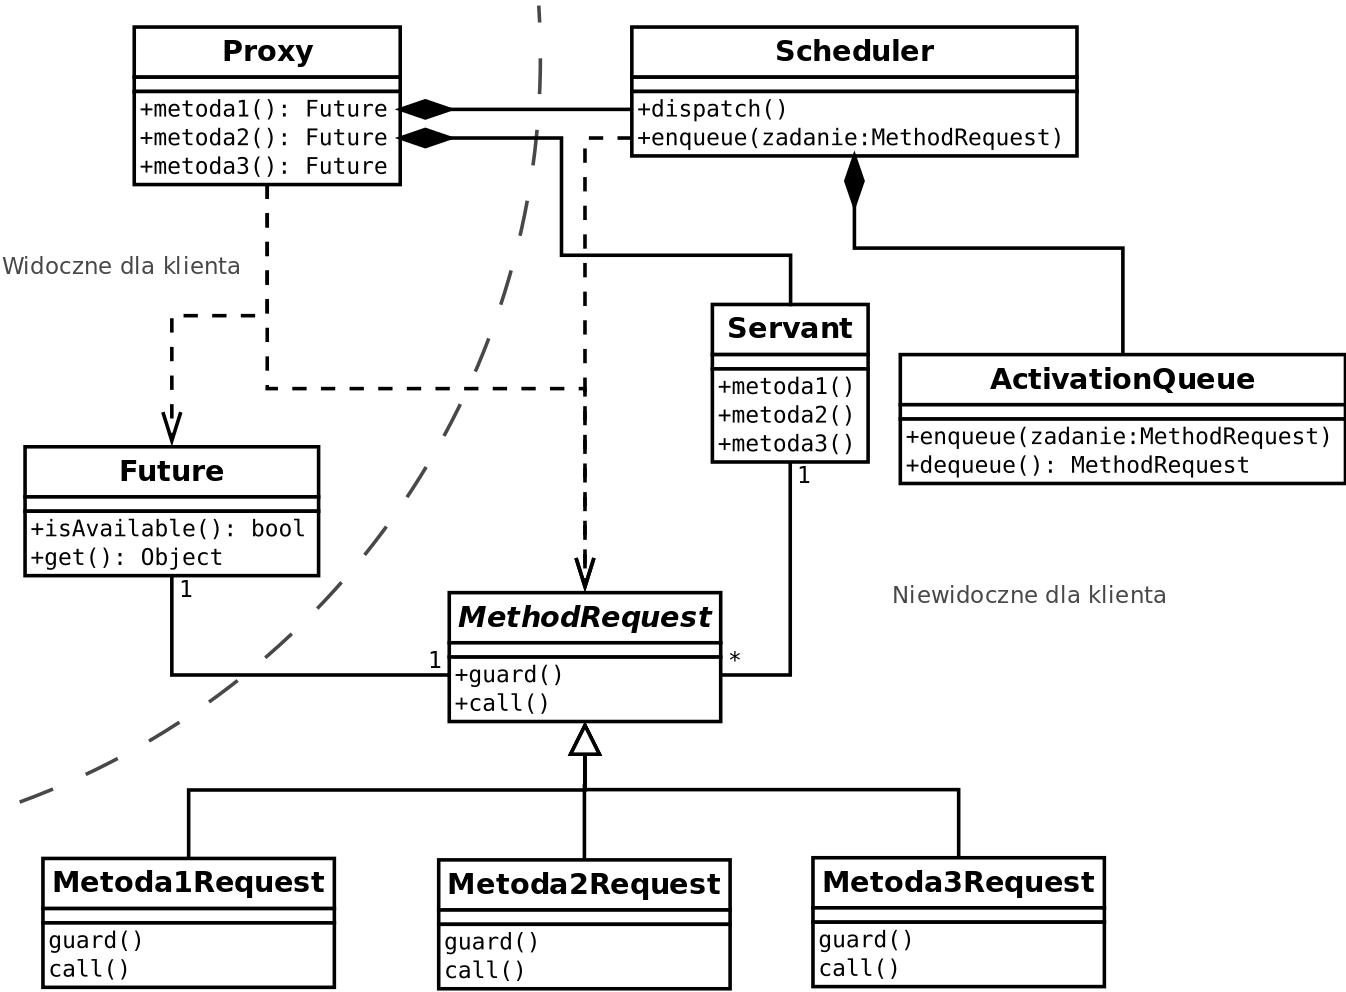
\includegraphics[width=0.5\textwidth]{./Active_object_pl.png}
\caption{Schemat wzroca Active Object}
\end{figure}


Wzorzec Active Object oddziela wykonywanie długotrwałych operacji od głównego
wątku, umożliwiając asynchroniczne przetwarzanie zadań. Zadania są umieszczane w
kolejce i wykonywane przez osobny wątek (serwant). Klient otrzymuje wynik
operacji za pomocą obiektu Future, który zostaje ''ukończony'' po
zakończeniu zadania.
Celem laboratorium było zaimplementowanie bufora, używając właśnie tego wzorca.
W tym celu będziemy implementować kolejne klasy z diagramu, lub też czasami
używać gotowych klas z biblioteki standardowej.
\subsection*{Klasa \texttt{Buffer} (Pracownik/Servant)}
\label{sec:org4c694f3}
Klasa ta jest odpowiedzialna za logikę bufora, czyli dodawanie i pobieranie
elementów z kolejki. Również znajdują się w niej metody umożliwiające sprawdzenie
czy dana operacja jest możliwa.

\begin{Code}
\begin{Verbatim}
\color{EFD}\EFk{class} \EFt{Buffer} \EFrda{\{}
    \EFk{private} \EFk{final} \EFt{int} \EFv{capacity};
    \EFk{private} \EFk{final} \EFt{List}\EFrdb{<}\EFt{Integer}\EFrdb{>} \EFv{buffer} = \EFk{new} \EFt{LinkedList}\EFrdb{<}\EFrdb{>}\EFrdb{(}\EFrdb{)};

    \EFk{public} Buffer\EFrdb{(}\EFt{int} \EFv{capacity}\EFrdb{)} \EFrdb{\{}
        \EFk{this}.capacity = capacity;
    \EFrdb{\}}

    \EFk{public} \EFt{void} \EFf{put}\EFrdb{(}\EFt{int} \EFv{value}\EFrdb{)} \EFrdb{\{}
        buffer.add\EFrdc{(}value\EFrdc{)};
    \EFrdb{\}}

    \EFk{public} \EFt{int} \EFf{get}\EFrdb{(}\EFrdb{)} \EFrdb{\{}
        \EFk{return} buffer.removeFirst\EFrdc{(}\EFrdc{)};
    \EFrdb{\}}

    \EFk{public} \EFt{boolean} \EFf{isEmpty}\EFrdb{(}\EFrdb{)} \EFrdb{\{}
        \EFk{return} buffer.isEmpty\EFrdc{(}\EFrdc{)};
    \EFrdb{\}}

    \EFk{public} \EFt{boolean} \EFf{isFull}\EFrdb{(}\EFrdb{)} \EFrdb{\{}
        \EFk{return} buffer.size\EFrdc{(}\EFrdc{)} == capacity;
    \EFrdb{\}}
\EFrda{\}}
\end{Verbatim}
\end{Code}
\subsection*{\texttt{MethodRequest}}
\label{sec:org3268bf8}
\texttt{MethodRequest} reprezentuje pojedyncze zadanie do wykonania, przechowując
informacje o metodzie i jej parametrach. Jest umieszczany w kolejce i
przetwarzany przez pracownika.
Poza metodą \texttt{call()} mamy również metodę \texttt{guard()} która sprawdza czy operacja może
być wykonana. Używamy tutaj \texttt{CompletableFuture}, aby poinformować klienta o
zakończeniu zadania.  Użycie gotowej klasy upraszcza implementację oraz
dostarcza użytkownikowi mnóstwo wygodnych metod do obsługi wyniku.
Klasa \texttt{MethodRequest} jest generyczna ze względu na typ zawarty w \texttt{CompletableFuture}.

Klasa abstrakcyjna \texttt{MethodRequest}:
\begin{Code}
\begin{Verbatim}
\color{EFD}\EFk{abstract} \EFk{class} \EFt{MethodRequest}\EFrda{<}\EFt{T}\EFrda{>} \EFrda{\{}
    \EFk{protected} \EFk{final} \EFt{Buffer} \EFv{buffer};
    \EFk{protected} \EFk{final} \EFt{CompletableFuture}\EFrdb{<}\EFt{T}\EFrdb{>} \EFv{future} = \EFk{new} \EFt{CompletableFuture}\EFrdb{<}\EFrdb{>}\EFrdb{(}\EFrdb{)};

    \EFk{public} MethodRequest\EFrdb{(}Buffer buffer\EFrdb{)} \EFrdb{\{}
        \EFk{this}.buffer = buffer;
    \EFrdb{\}}

    \EFk{public} \EFk{abstract} \EFt{void} \EFf{execute}\EFrdb{(}\EFrdb{)};

    \EFk{public} \EFk{abstract} \EFt{boolean} \EFf{guard}\EFrdb{(}\EFrdb{)};
\EFrda{\}}
\end{Verbatim}
\end{Code}
\subsubsection*{\texttt{PutRequest}}
\label{sec:orgfa2afb8}
\begin{Code}
\begin{Verbatim}
\color{EFD}\EFk{class} \EFt{PutRequest} \EFk{extends} \EFt{MethodRequest}\EFrda{<}\EFt{Void}\EFrda{>} \EFrda{\{}
    \EFk{private} \EFk{final} \EFt{int} \EFv{value};

    \EFk{public} PutRequest\EFrdb{(}\EFt{Buffer} \EFv{buffer}, \EFt{int} \EFv{value}\EFrdb{)} \EFrdb{\{}
        \EFk{super}\EFrdc{(}buffer\EFrdc{)};
        \EFk{this}.value = value;
    \EFrdb{\}}

    \textcolor[HTML]{008b8b}{@Override}
    \EFk{public} \EFt{void} \EFf{execute}\EFrdb{(}\EFrdb{)} \EFrdb{\{}
        System.out.println\EFrdc{(}\EFs{"PUT REQUEST "} + value\EFrdc{)};
        buffer.put\EFrdc{(}value\EFrdc{)};
        future.complete\EFrdc{(}\EFo{null}\EFrdc{)};
    \EFrdb{\}}

    \textcolor[HTML]{008b8b}{@Override}
    \EFk{public} \EFt{boolean} \EFf{guard}\EFrdb{(}\EFrdb{)} \EFrdb{\{}
        \EFk{return} \EFnc{!}buffer.isFull\EFrdc{(}\EFrdc{)};
    \EFrdb{\}}
\EFrda{\}}
\end{Verbatim}
\end{Code}
\subsubsection*{\texttt{GetRequest}}
\label{sec:org0b1a5c4}
\begin{Code}
\begin{Verbatim}
\color{EFD}\EFk{class} \EFt{GetRequest} \EFk{extends} \EFt{MethodRequest}\EFrda{<}\EFt{Integer}\EFrda{>} \EFrda{\{}
    \EFk{public} GetRequest\EFrdb{(}Buffer buffer\EFrdb{)} \EFrdb{\{}
        \EFk{super}\EFrdc{(}buffer\EFrdc{)};
    \EFrdb{\}}

    \textcolor[HTML]{008b8b}{@Override}
    \EFk{public} \EFt{void} \EFf{execute}\EFrdb{(}\EFrdb{)} \EFrdb{\{}
        System.out.println\EFrdc{(}\EFs{"GET REQUEST"}\EFrdc{)};
        future.complete\EFrdc{(}buffer.get\EFrdd{(}\EFrdd{)}\EFrdc{)};
    \EFrdb{\}}

    \textcolor[HTML]{008b8b}{@Override}
    \EFk{public} \EFt{boolean} \EFf{guard}\EFrdb{(}\EFrdb{)} \EFrdb{\{}
        \EFk{return} \EFnc{!}buffer.isEmpty\EFrdc{(}\EFrdc{)};
    \EFrdb{\}}
\EFrda{\}}
\end{Verbatim}
\end{Code}
\subsection*{\texttt{Scheduler}}
\label{sec:orgd0a6c77}
\texttt{Scheduler} zajmuje się wrzucaniem obiektów \texttt{MethodRequest} do kolejki.
Odpowiada on również za pobieranie tych obiektów z kolejki i uruchamianie ich.
Zamiast dedykowanej klasy na kolejkę, używamy gotowej klasy \texttt{ConcurrentLinkedQueue}.
Kod klasy \texttt{Scheduler}, jest bardzo prosty. Metoda \texttt{run()} jest wykonywana
w osobnym wątku od klienta i zarówno pobiera zadania z kolejki, jak i je wykonuje.
Gdy zadanie nie może być wykonane, jest ono ponownie dodawane do kolejki.


\begin{Code}
\begin{Verbatim}
\color{EFD}\EFk{class} \EFt{Scheduler} \EFrda{\{}
    \EFk{private} \EFk{final} \EFt{Queue}\EFrdb{<}\EFt{MethodRequest}\EFrdc{<}?\EFrdc{>}\EFrdb{>} \EFv{requests} = \EFk{new} \EFt{ConcurrentLinkedQueue}\EFrdb{<}\EFrdb{>}\EFrdb{(}\EFrdb{)};

    \EFk{public} \EFt{void} \EFf{enqueue}\EFrdb{(}\EFt{MethodRequest}\EFrdc{<}?\EFrdc{>} \EFv{request}\EFrdb{)} \EFrdb{\{}
        requests.add\EFrdc{(}request\EFrdc{)};
    \EFrdb{\}}

    \EFk{public} \EFt{void} \EFf{run}\EFrdb{(}\EFrdb{)} \EFrdb{\{}
        \EFk{while} \EFrdc{(}\EFo{true}\EFrdc{)} \EFrdc{\{}
            \EFt{MethodRequest}\EFrdd{<}?\EFrdd{>} \EFv{request} = requests.poll\EFrdd{(}\EFrdd{)};
            \EFk{if} \EFrdd{(}request != \EFo{null}\EFrdd{)} \EFrdd{\{}
                \EFk{if} \EFrda{(}request.guard\EFrdb{(}\EFrdb{)}\EFrda{)} \EFrda{\{}
                    request.execute\EFrdb{(}\EFrdb{)};
                \EFrda{\}} \EFk{else} \EFrda{\{}
                    requests.add\EFrdb{(}request\EFrdb{)};
                \EFrda{\}}
            \EFrdd{\}}
        \EFrdc{\}}
    \EFrdb{\}}
\EFrda{\}}
\end{Verbatim}
\end{Code}
\subsection*{\texttt{BufferProxy}}
\label{sec:org3867074}
\texttt{BufferProxy} jest klasą, która jest używana przez klienta.
Jej interfejs jest bardzo podobny do interfejsu klasy \texttt{Buffer}, ale zamiast
wyników bezpośrednich \texttt{void} / \texttt{int} zwraca obiekty \texttt{CompletableFuture}, przez
to używanie takiej klasy jest bardzo intuicyjne.
Klasa \texttt{BufferProxy} uruchamiania wątek scheduler'a, oraz tworzy odpowiednie obiekty
\texttt{MethodRequest} i przekazuje je do \texttt{Scheduler}.

\begin{Code}
\begin{Verbatim}
\color{EFD}\EFk{class} \EFt{BufferProxy} \EFrda{\{}
    \EFk{private} \EFk{final} \EFt{Scheduler} \EFv{scheduler} = \EFk{new} \EFt{Scheduler}\EFrdb{(}\EFrdb{)};
    \EFk{private} \EFk{final} \EFt{Buffer} \EFv{buffer};

    \EFk{public} BufferProxy\EFrdb{(}\EFt{int} \EFv{capacity}\EFrdb{)} \EFrdb{\{}
        \EFk{this}.buffer = \EFk{new} \EFt{Buffer}\EFrdc{(}capacity\EFrdc{)};

        \EFt{var} \EFv{thread} = \EFk{new} \EFt{Thread}\EFrdc{(}scheduler::run\EFrdc{)};
        thread.setDaemon\EFrdc{(}\EFo{true}\EFrdc{)};
        thread.start\EFrdc{(}\EFrdc{)};
    \EFrdb{\}}

    \EFk{public} \EFt{CompletableFuture}\EFrdb{<}\EFt{Void}\EFrdb{>} \EFf{put}\EFrdb{(}\EFt{int} \EFv{value}\EFrdb{)} \EFrdb{\{}
        \EFt{var} \EFv{request} = \EFk{new} \EFt{PutRequest}\EFrdc{(}buffer, value\EFrdc{)};
        scheduler.enqueue\EFrdc{(}request\EFrdc{)};
        \EFk{return} request.future;
    \EFrdb{\}}

    \EFk{public} \EFt{CompletableFuture}\EFrdb{<}\EFt{Integer}\EFrdb{>} \EFf{get}\EFrdb{(}\EFrdb{)} \EFrdb{\{}
        \EFt{var} \EFv{request} = \EFk{new} \EFt{GetRequest}\EFrdc{(}buffer\EFrdc{)};
        scheduler.enqueue\EFrdc{(}request\EFrdc{)};
        \EFk{return} request.future;
    \EFrdb{\}}
\EFrda{\}}
\end{Verbatim}
\end{Code}
\section*{Przykład użycia}
\label{sec:org46eeb2e}
Implementujemy dwie klasy \texttt{Producer} i \texttt{Consumer}.
Wykonują swoje operacje w pętli, ale po każdej operacji \textbf{nie} czekają
na zakończenie operacji. Po wykoaniu całej pętli, wątki czekają aż wszystkie
ich wysłane zadania zostały zakończone.
\subsection*{\texttt{Producer}}
\label{sec:org5d9b6e9}
\begin{Code}
\begin{Verbatim}
\color{EFD}\EFk{class} \EFt{Producer} \EFk{implements} \EFt{Runnable} \EFrda{\{}
    \EFk{private} \EFk{final} \EFt{int} \EFv{toProduce};
    \EFk{private} \EFk{final} \EFt{BufferProxy} \EFv{buffer};
    \EFk{private} \EFk{final} \EFt{int} \EFv{id};

    \EFk{public} Producer\EFrdb{(}\EFt{int} \EFv{id}, \EFt{int} \EFv{toProduce}, BufferProxy buffer\EFrdb{)} \EFrdb{\{}
        \EFk{this}.id = id;
        \EFk{this}.toProduce = toProduce;
        \EFk{this}.buffer = buffer;
    \EFrdb{\}}

    \textcolor[HTML]{008b8b}{@Override}
    \EFk{public} \EFt{void} \EFf{run}\EFrdb{(}\EFrdb{)} \EFrdb{\{}
        \EFt{List}\EFrdc{<}\EFt{CompletableFuture}\EFrdd{<}\EFt{Void}\EFrdd{>}\EFrdc{>} \EFv{futures} = \EFk{new} \EFt{ArrayList}\EFrdc{<}\EFrdc{>}\EFrdc{(}\EFrdc{)};
        \EFk{for} \EFrdc{(}\EFt{int} \EFv{i} = \EFhn{0}; i < \EFt{toProduce}; i++\EFrdc{)} \EFrdc{\{}
            futures.add\EFrdd{(}buffer.put\EFrda{(}i\EFrda{)}\EFrdd{)};

            \EFk{try} \EFrdd{\{}
                Thread.sleep\EFrda{(}\EFhn{30}\EFrda{)};
            \EFrdd{\}} \EFk{catch} \EFrdd{(}InterruptedException e\EFrdd{)} \EFrdd{\{}
                e.printStackTrace\EFrda{(}\EFrda{)};
            \EFrdd{\}}
        \EFrdc{\}}

        System.out.printf\EFrdc{(}\EFs{"Producer \%d finished sending requests\%n"}, id\EFrdc{)};
        CompletableFuture.allOf\EFrdc{(}futures.toArray\EFrdd{(}\EFk{new} \EFt{CompletableFuture}\EFrda{[}\EFhn{0}\EFrda{]}\EFrdd{)}\EFrdc{)}.join\EFrdc{(}\EFrdc{)};
        System.out.printf\EFrdc{(}\EFs{"Producer \%d: all actions have been done\%n"}, id\EFrdc{)};
    \EFrdb{\}}
\EFrda{\}}
\end{Verbatim}
\end{Code}
\subsection*{\texttt{Consumer}}
\label{sec:org0f531d9}
\begin{Code}
\begin{Verbatim}
\color{EFD}\EFk{class} \EFt{Consumer} \EFk{implements} \EFt{Runnable} \EFrda{\{}
    \EFk{private} \EFk{final} \EFt{int} \EFv{toConsume};
    \EFk{private} \EFk{final} \EFt{BufferProxy} \EFv{buffer};
    \EFk{private} \EFk{final} \EFt{int} \EFv{id};

    \EFk{public} Consumer\EFrdb{(}\EFt{int} \EFv{id}, \EFt{int} \EFv{toConsume}, BufferProxy buffer\EFrdb{)} \EFrdb{\{}
        \EFk{this}.id = id;
        \EFk{this}.toConsume = toConsume;
        \EFk{this}.buffer = buffer;
    \EFrdb{\}}

    \textcolor[HTML]{008b8b}{@Override}
    \EFk{public} \EFt{void} \EFf{run}\EFrdb{(}\EFrdb{)} \EFrdb{\{}
        \EFt{List}\EFrdc{<}\EFt{CompletableFuture}\EFrdd{<}\EFt{Integer}\EFrdd{>}\EFrdc{>} \EFv{futures} = \EFk{new} \EFt{ArrayList}\EFrdc{<}\EFrdc{>}\EFrdc{(}\EFrdc{)};
        \EFk{for} \EFrdc{(}\EFt{int} \EFv{i} = \EFhn{0}; i < \EFt{toConsume}; i++\EFrdc{)} \EFrdc{\{}
            futures.add\EFrdd{(}buffer.get\EFrda{(}\EFrda{)}\EFrdd{)};

            \EFk{try} \EFrdd{\{}
                Thread.sleep\EFrda{(}\EFhn{30}\EFrda{)};
            \EFrdd{\}} \EFk{catch} \EFrdd{(}InterruptedException e\EFrdd{)} \EFrdd{\{}
                e.printStackTrace\EFrda{(}\EFrda{)};
            \EFrdd{\}}
        \EFrdc{\}}

        System.out.printf\EFrdc{(}\EFs{"Consumer \%d finished sending requests\%n"}, id\EFrdc{)};

        \EFt{var} \EFv{results} = futures.stream\EFrdc{(}\EFrdc{)}
                 .map\EFrdc{(}CompletableFuture::join\EFrdc{)}
                 .map\EFrdc{(}String::valueOf\EFrdc{)}
                 .collect\EFrdc{(}Collectors.joining\EFrdd{(}\EFs{", "}\EFrdd{)}\EFrdc{)};
        System.out.printf\EFrdc{(}\EFs{"Consumer \%d: received values: \%s\%n"}, id, results\EFrdc{)};

        System.out.printf\EFrdc{(}\EFs{"Consumer \%d: all actions have been done\%n"}, id\EFrdc{)};
    \EFrdb{\}}

\EFrda{\}}
\end{Verbatim}
\end{Code}
\subsection*{Funkcja \texttt{main}}
\label{sec:org711cb5f}
\begin{Code}
\begin{Verbatim}
\color{EFD}\EFk{public} \EFk{static} \EFt{void} \EFf{main}\EFrda{(}\EFt{String}\EFrdb{[}\EFrdb{]} \EFv{args}\EFrda{)} \EFk{throws} \EFt{ExecutionException}, \EFt{InterruptedException} \EFrda{\{}
    \EFt{BufferProxy} \EFv{buffer} = \EFk{new} \EFt{BufferProxy}\EFrdb{(}\EFhn{5}\EFrdb{)};

    \EFt{var} \EFv{producers} = IntStream.range\EFrdb{(}\EFhn{0}, \EFhn{3}\EFrdb{)}
            .mapToObj\EFrdb{(}i -> \EFk{new} \EFt{Producer}\EFrdc{(}i, \EFhn{10}, buffer\EFrdc{)}\EFrdb{)}
            .map\EFrdb{(}Thread::\EFk{new}\EFrdb{)}
            .toList\EFrdb{(}\EFrdb{)};
    \EFt{var} \EFv{consumers} = IntStream.range\EFrdb{(}\EFhn{0}, \EFhn{2}\EFrdb{)}
            .mapToObj\EFrdb{(}i -> \EFk{new} \EFt{Consumer}\EFrdc{(}i, \EFhn{15}, buffer\EFrdc{)}\EFrdb{)}
            .map\EFrdb{(}Thread::\EFk{new}\EFrdb{)}
            .toList\EFrdb{(}\EFrdb{)};

    \EFk{try} \EFrdb{(}\EFt{var} \EFv{executor} = Executors.newFixedThreadPool\EFrdc{(}\EFhn{7}\EFrdc{)}\EFrdb{)} \EFrdb{\{}
        producers.forEach\EFrdc{(}executor::submit\EFrdc{)};
        consumers.forEach\EFrdc{(}executor::submit\EFrdc{)};

        executor.shutdown\EFrdc{(}\EFrdc{)};
        \EFt{boolean} \EFv{terminated} = executor.awaitTermination\EFrdc{(}\EFhn{1}, \EFo{TimeUnit}.MINUTES\EFrdc{)};
        \EFk{if} \EFrdc{(}terminated\EFrdc{)} \EFrdc{\{}
            System.out.println\EFrdd{(}\EFs{"All threads have finished"}\EFrdd{)};
        \EFrdc{\}} \EFk{else} \EFrdc{\{}
            System.out.println\EFrdd{(}\EFs{"Program has timed out"}\EFrdd{)};
        \EFrdc{\}}
    \EFrdb{\}}
\EFrda{\}}
\end{Verbatim}
\end{Code}
\subsection*{Wynik programu}
\label{sec:org589d2e2}
\begin{tcolorbox}
\begin{Verbatim}
PUT REQUEST 0
PUT REQUEST 0
GET REQUEST
PUT REQUEST 0
GET REQUEST
PUT REQUEST 1
PUT REQUEST 1
PUT REQUEST 1
GET REQUEST
GET REQUEST
PUT REQUEST 2
GET REQUEST
GET REQUEST
PUT REQUEST 2
PUT REQUEST 2
GET REQUEST
PUT REQUEST 3
PUT REQUEST 3
GET REQUEST
PUT REQUEST 3
PUT REQUEST 4
GET REQUEST
PUT REQUEST 4
GET REQUEST
PUT REQUEST 4
GET REQUEST
PUT REQUEST 5
GET REQUEST
PUT REQUEST 5
GET REQUEST
GET REQUEST
PUT REQUEST 6
PUT REQUEST 5
GET REQUEST
PUT REQUEST 7
GET REQUEST
PUT REQUEST 7
GET REQUEST
PUT REQUEST 6
GET REQUEST
PUT REQUEST 8
\end{Verbatim}


\end{tcolorbox}\begin{tcolorbox}
\begin{Verbatim}
GET REQUEST
PUT REQUEST 9
GET REQUEST
PUT REQUEST 9
GET REQUEST
Producer 1 finished sending requests
Producer 2 finished sending requests
Producer 0 finished sending requests
Producer 0: all actions have been done
PUT REQUEST 6
GET REQUEST
PUT REQUEST 8
GET REQUEST
PUT REQUEST 8
GET REQUEST
PUT REQUEST 7
Producer 2: all actions have been done
GET REQUEST
PUT REQUEST 9
GET REQUEST
Producer 1: all actions have been done
GET REQUEST
GET REQUEST
GET REQUEST
GET REQUEST
Consumer 0 finished sending requests
Consumer 1 finished sending requests
Consumer 1: received values: 0, 0, 1, 2, 3, 3, 4, 5, 5, 7, 6, 9, 6, 8, 7
Consumer 1: all actions have been done
Consumer 0: received values: 0, 1, 1, 2, 2, 3, 4, 4, 6, 5, 7, 8, 9, 8, 9
Consumer 0: all actions have been done
All threads have finished
\end{Verbatim}


\end{tcolorbox}Wszystkie wątki zakończyły swoje działanie, a wyniki są zgodne z oczekiwaniami.
Występuję bardzo naturalny przeplot operacji \texttt{PUT} i \texttt{GET}.
\section*{Wnioski}
\label{sec:org62f1bce}
Implementacja wzorca Active Object w kontekście problemu producent-konsument
pozwoliła na skuteczną separację logiki operacji (dodawania i pobierania
elementów z bufora) od synchronizacji wątków. Klasy \texttt{CompletableFuture} i
\texttt{BufferProxy} tworzą wygodny interfejs do interkacji z buforem.

Wynikiem zastosowania wzorca Active Object jest świetny kod z punktu widzenia
klienta, który nie musi martwić się o detale współbieżności.
Trzeba natomiast zwrócić uwagę na to, że wzorzec ten jest stosunkowo kosztowny
w implementacji, a co za tym idzie w utrzymaniu. Dla prostych problemów
może być on wysoce nadmiarowy. Trzeba też zwrócić uwagę na to dodatkowy
koszt związany z tym wzorcem, który wynika m.in. z konieczności tworzenia obiektów
\texttt{MethodRequest}. Dla obszarów gdzie wydajność jest kluczowa, warto zastanowić się
czy ten wzorzec jest odpowiedni.


Wzorzec Active Object może być świetnym wyborem np. gdy piszemy bibliotekę,
bo dzięki niemu jej użytkownicy otrzymają wygodny interfejs oraz odsperowanie
problemów związanych z wielowątkowością.
\section*{Bibliografia}
\label{sec:orgd55fe5a}
\begin{itemize}
\item \href{https://pl.wikipedia.org/wiki/Active\_object}{Active Object - Wikipedia}
\end{itemize}
\end{document}
